\chapter{Questions and interrogatives} \label{ch:questions}

\epigraph{every answer\\
carries within it\\
the ghost of its question}{}

Questions\is{question|(} feature prominently in education, no less so in language learning classrooms. Most of them are asked by teachers to students, and many are experienced as awkward by students because of a feeling that the answer\is{answer|(} is obvious. Consider the following interaction reproduced from \citet[23]{nunn1999purposes}.

\ea
\textbf{T:} \textit{And then we know that Mr Archer came on his own before... without
anybody. He left his family in England and he came on his own to the
Gulf. So he had to look for a house to live in first before he starts
anything else and as you know he has found a house. And this
house... who can tell me something about this house?
What does does this house consist of? Tell me about this house.
Yes, Mohanned.}\\
\textbf{S:} \textit{It's a villa with a large garden.}\\
\textbf{T:} \textit{Yes. It's a villa with a large garden. That's right.}\\
\z

I don't know about you, but I find this painful to read. Good on Mohanned for helping everyone get on with things, but yeesh! What was the teacher thinking? To be frank, it was probably something like, ``I've been talking a lot. Maybe I should give the students a chance,'' at which point, the question just popped out. 

But what was achieved? If the goal was to offer the students an opportunity to practice speaking, this seems wholly insufficient. In a class of who knows how many students, one said an eight-word (eight-token, see Section \ref{sec:family-lemma-shape-token}) sentence that took all of, perhaps, three seconds, before the speaking turn reverted to the teacher. Nor was it likely to clarify the meaning of the text; the teacher even says, ``as you know,'' so, was anyone even confused about the nature of the house?  And, really, did it matter if they were? It could have been a bungalow or an apartment for all the difference it made to the educational value of the interaction.

As John \citet{searle1969} observed, we do things with language, and questioning is one kind of thing we do. But in this case, it's akin to asking a guest if they would like a seat when they are already comfortably seated. Such a question is not just redundant but also disrupts the flow of social interaction, highlighting a disconnect between the speaker's intention and the situation. Similarly, in the classroom, the teacher's question, though well-intentioned, ends up creating an awkward moment that does little to advance the educational or social dynamics of the setting.

Of course, it's not quite as cringe-worthy as the seat offer would be. There's a script playing out here, and both the students and the teacher know how it's supposed to go. But that only goes some way to reducing the awkwardness of this meaningless question\is{question|)}, and it doesn't mean that anybody needs to be happy about their role in the farce.

A key insight about the language landscape is that, in focusing on language forms, we risk overlooking the crux of communication: its purpose. Different forms have different purposes; in Searle's words, they perform \textsc{speech acts}. Fostering a classroom environment where students partake in genuine and natural speech acts leads to a more positive and comfortable learning experience.

\section{Questions vs interrogatives}

A \textsc{question}\is{question|(} is something that asks for an answer\is{answer|)}, whether it gets one or not. But questions are not all linguistic. Sure, they're typically speech acts, or things we do with language, but they don't have to be. If you walk into your kitchen and find a gift on your table, this might pose a number of questions, questions about its source and contents, perhaps about the intended recipient or even about the method of delivery. These don't even have to be formulated into language, let alone uttered to be questions.

Of course we often do use language to ask questions. The most common way to do so is through the use of an \textsc{interrogative clause}\is{interrogative clause|(} such as \textit{What's that gift doing there?} and \textit{Is it for me?} (Later in the book we'll deal with subordinate clauses~-- those that appear inside larger clauses~-- but for now, we'll focus on main-clause interrogatives.) Recalling the discussion of the many-to-many relationships between categories and functions in Section \ref{sec:many-to-many}, we find the same kind of relationship with interrogatives\is{interrogative clause!and clause type} and questions\is{question!and interrogatives}. As the gift example illustrates, questions don't have to be in the form of interrogatives; they don't even have to be linguistic. But, even if they are expressed in language, they can take non-interrogative forms. \textit{That's for me?} is a question (hence the question mark), but not an interrogative clause. You could even just ask \textit{for me?} which isn't even a clause, let alone an interrogative.

Conversely, an interrogative doesn't have to be a question\is{question|)}. It could be a threat (\textit{do you want to try that again?}), an offer (\textit{how would you like some help?}), an instruction (\textit{why don't you try again?}), an evaluation (\textit{is that the best you can do?}), or any number of other speech acts.

\begin{tcolorbox}[title=Terminological hygiene, colback=white, parbox]\label{box:terminology-hygiene}
\setlength{\parindent}{1.5em}
    \noindent As I've pointed out a number of times, words (almost) never have a single correct meaning. Obviously, \textit{cookie} does not mean `in an upwards direction', but it does mean `a small file stored on a user's computer by a web browser for tracking or data retrieval purposes' as well as `a sweet baked treat, often containing ingredients such as chocolate, nuts, or raisins'. I've also taken pains to make clear that just because a term such as \textsc{phrase} has a technical meaning along with non-technical meanings, it's not true that the non-technical meaning is generally wrong. It just depends on what one means: In the appropriate technical environment, the technical meaning should take priority.
    
    That said, careless use of terminology often leads to confusion. One common problem in discussions of language is re-using terms dealing with diverse aspects of language. For instance, in the field of semantics, \textit{subject}\is{subject (Subj)!|(} means `the main topic or the primary entity that the statement is about', but for the syntactician it means `the function of a constituent in a clause that normally precedes the verb and, in active clauses, normally denotes the actor (if there is one) but in passive clauses, normally denotes whatever is acted upon'. This can be a problem.
    
    Technical terms are often drawn from existing words. Instead of making up a totally new one like \textit{predicore} or \textit{maintent} to denote the technical meaning that syntacticians and semanticists have in mind when they use \textit{subject}, both fields draw on the same non-technical vocabulary. The result is that many people coming to linguistics or language teaching for the first time are confused.
    
    Another example of such confusing teminological overlap is \textsc{predicate}, which, in syntax refers to `the VP that is the \textsf{Head} of the clause', while in semantics, means `a relation or property that is ascribed to one or more entities'.\footnote{It's the conceptual meaning or function that links the semantic subject to some assertion or description about it. In the example \textit{the cat sleeps}, the semantic predicate is the concept of sleeping that is attributed to the entity cat.}

    I've avoided this kind of overlapping terminology here, and I encourage you to do so in your teaching too, within reason. This is just to avoid confusion, not because certain uses of terms are correct or incorrect. So, whenever I use the term \textsc{question}, for example, I mean it semantically, and whenever I used \textsc{interrogative}, I mean it syntactically.
\end{tcolorbox}

\section{Main-clause interrogatives}

Main-clause interrogatives\footnote{As I mentioned, subordinate interrogative clauses\is{interrogative clause!subordinate}, like \textit{I wonder \uline{who it could be}}, will be dealt with in a later chapter.} can be broadly divided into those with an interrogative word (e.g., \textit{\uline{What} is it?}) and those without (\textit{Could it be a platypus?}). I'll use the terms \textsc{focused}\is{interrogative clause!basic vs focused|(} for those that include an interrogative word and \textsc{basic} for the others that start with an auxiliary verb.\footnote{\textit{CGEL} uses \textsc{open} and \textsc{closed} for these interrogative types, but since those terms describe semantic question types (see Section \ref{sec:question-semantics}), applying them to syntactic forms can be misleading. This chapter therefore uses \textsc{basic} and \textsc{focused} to describe the form of the clauses.}

\section{Basic interrogatives}\label{sec:basic-int}

Basic interrogatives invert the typical subject--verb order: The declarative \textit{Today is a lovely day} becomes the basic interrogative \textit{Is today a lovely day?} 

\begin{figure}
    \centering
    \begin{tikzpicture}[node distance=1cm]
    % Nodes for the declarative sentence
    \node (today1) {\textit{Today}};
    \node[right=of today1] (is1) {\textit{is}};
    \node[right=of is1] (a1) {\textit{a}};
    \node[right=of a1] (lovely1) {\textit{lovely}};
    \node[right=of lovely1] (day1) {\textit{day.}};

    % Nodes for the interrogative sentence
    \node[below=of today1] (is2) {\textit{Is}};
    \node[right=of is2] (today2) {\textit{today}};
    \node[right=of today2] (a2) {\textit{a}};
    \node[right=of a2] (lovely2) {\textit{lovely}};
    \node[right=of lovely2] (day2) {\textit{day?}};

    % Arrows
    \draw[->, thick] (is1) -- (is2) node [pos=0.5,left] {};
    \draw[->, thick] (today1.south) -- ++(0,-0.5) -| (today2.north);

\end{tikzpicture}
    \caption{The subject and the auxiliary verb \textit{is} switch places in the basic interrogative.}
    \label{fig:subj-aux-inversion}
\end{figure}

Not just any verb can participate in this inversion, only auxiliary verbs\is{auxiliary verb|(}\is{auxiliary verb!and inversion|(}. In contemporary English, you can ask \textit{Are they going?} with the auxiliary verb \textit{are} in front of the subject \textit{they} but not *\textit{Go they?} with the lexical verb \textit{go} in front.\footnote{\textit{Go they} was possible until the end of the eighteenth century \citep[239]{Lass1999}.}

I introduced the auxiliary verbs in Section \ref{sec:aux} as those that have the NICER properties, and this kind of inversion is the \textit{I} in NICER (see Table \ref{tab:NICER2}).

\begin{table}
    \centering
    \begin{tabularx}{0.80\textwidth}{@{} >{\centering\arraybackslash\hsize=.03\hsize}X >{\hsize=.21\hsize}X >{\hsize=.38\hsize}X >{\hsize=.38\hsize}X @{}}
    \multicolumn{2}{>{\hsize=.24\hsize}X}{\textbf{Feature}} & \textbf{Examples} & \textbf{Counter-Examples} \\
    \hline
    \textbf{N} & egation:& \textit{Lee \uline{will} not eat.} & *\textit{Lee eats not.} \\
    \rowcolor{gray!20} % Apply background color here
    \textbf{I} & nversion:& \textit{Lee \uline{has} eaten.} \(\rightarrow\) \newline \textit{\uline{Has} Lee eaten?} & *\textit{Eats Lee?} \\
    \textbf{C} & ontraction:& \textit{didn't}, \textit{shouldn't} & *\textit{eatn't}, *\textit{keptn't} \\
    \textbf{E} & llipsis:& \textit{Kim \uline{was} eating, and \newline Lee \uline{was} ..., too.} & *\textit{Kim kept eating, and \newline Lee kept ..., too.} \\
    \textbf{R} & ebuttal:& \textit{I did tóo}/\textit{só read it.} \newline (\textit{Did not!}) & *\textit{I tried tóo}/\textit{só to read it.} (\textit{Tried not!}) \\
\end{tabularx}
\caption{The NICER properties}\label{tab:NICER2}
\end{table}

\is{auxiliary verb!NICER properties}The other part of the inversion is the subject\is{subject (Subj)!and inversion|(}, which is introduced in Section \ref{sec:subjects}. There, I mentioned that \textsf{Subjects} typically precede the \textsf{Head} VP, but that in a basic interrogative (\textit{Could \uline{they} be right?}), the subject comes immediately after an auxiliary verb. \textsf{Subject}--auxiliary inversion\is{inversion!subject--auxiliary|(}\is{subject--auxiliary inversion|(} is a key aspect of basic interrogatives, and that's actually kinda weird. Most languages don't make questions this way, and many language learners struggle with it. Instead of asking \textit{Is this right?} they'll ask \textit{This is right?} And of course, that's perfectly clear in most contexts, though, by default, it has the pragmatic force of requesting a clarification or expressing a doubt, rather than that of questioning.

\begin{tcolorbox}[title=Identifying the subject, colback=white, parbox]\label{box:finding-subject}
\setlength{\parindent}{1.5em}
    \noindent Sometimes, it's hard to find the subject. When you're stuck, alternating between a declarative and a basic interrogative can be helpful. Consider (\ref{ex:finding-subjects1} \& \ref{ex:finding-subjects2}).

    \ea \label{ex:finding-subjects1}
    \ea \textit{\uline{Tuesday} could be a good day to fly to Paris.}
        \ex \textit{Could \uline{Tuesday} be a good day to fly to Paris?}
        \z
    \z
    \ea \label{ex:finding-subjects2}
        \ea \textit{Tuesday, if things work out, \uline{you} could fly to Paris.}
        \ex \textit{Tuesday, if things work out, could \uline{you} fly to Paris?}
        \z
    \z

    In (\ref{ex:finding-subjects1}a), the first verb is the past-tense modal auxiliary \textit{could}. Modal auxiliaries don't have third-person singular forms, even in the present, and this is the past. As a result, agreement provides no clues about the subject. But in the basic interrogative in (\ref{ex:finding-subjects1}b), \textit{could} has moved in front of \textit{Tuesday}, which almost certainly means that \textit{Tuesday} is the subject.
    
    (\ref{ex:finding-subjects2}a) also lacks any agreement signals about the subject. But in the basic interrogative in (\ref{ex:finding-subjects2}b), \textit{could} is in front of \textit{you}, which means that \textit{Tuesday} \uline{cannot} be the subject; it must be \textit{you}.
    
\end{tcolorbox}

Here are some more examples with the auxiliary double underlined and the subject underlined. Those in (\ref{ex:befirstinterrogatives}) show different forms of auxiliary \textit{be}, those in (\ref{ex:modalfirstinterrogatives}) show different modal auxiliary verbs, and those in (\ref{ex:havefirstinterrogatives}) show two forms of auxiliary \textit{have} (as opposed to the lexical verb \textit{have}).
\ea \label{ex:befirstinterrogatives}
    \ea \textit{\uuline{Is} \uline{rain} ever warm?}
        \ex \textit{\uuline{Are} \uline{the evenings} sometimes too bright?}
        \ex \textit{\uuline{Am} \uline{I} functioning normally?}
        \ex \textit{Last night, \uuline{was} \uline{the moon}, perhaps, broken?}
    \z
\z
\ea \label{ex:modalfirstinterrogatives}
    \ea \textit{\uuline{Will} \uline{mornings} ever surprise you?}
        \ex \textit{\uuline{Could} \uline{silence} be too loud?}
    \z
\z
\ea\label{ex:havefirstinterrogatives}
    \ea \textit{In your experience, \uuline{have} \uline{dreams} lost their way?} 
    \ex \textit{\uuline{Had} \uline{the silent night} revealed its secrets before?} 
    \z
\z

You can see from these examples that, even with inversion, the auxiliary verb still agrees with the person and number of the subject, when possible: \textit{is} is the right form to agree with singular \textit{rain}, \textit{are} for plural \textit{the evenings}, and \textit{am} for first-person singular \textit{I}. 

I included (\ref{ex:befirstinterrogatives}d) to show that the auxiliary verb\is{auxiliary verb!position of|(} doesn't necessarily appear as the first element of the clause; other elements~-- the NP \textit{last night}, in this case~-- may come before it. The the auxiliary verb appears before the subject, but not always before everything. The same is true in (\ref{ex:havefirstinterrogatives}a): the auxiliary precedes the subject, but it still follows the PP \textit{in your experience}.


\subsection{\textit{Do} support}\label{sec:basic-do-support}

In all the examples so far, both the interrogative clauses and their corresponding declaratives would have an auxiliary verb. For example, the declarative counterpart of (\ref{ex:modalfirstinterrogatives}a) is \textit{Mornings \uline{will} {\op}sometimes{\cp} surprise you}, with the modal auxiliary verb \textit{will}. But lots of declarative clauses~-- perhaps most~-- don't have an auxiliary verb available for subject--auxiliary inversion. In such cases, we recruit \textit{do}, in its appropriate form. This is called \textsc{\textit{do} support}\is{do-support@\textit{do}-support|(}\is{auxiliary do@auxiliary \textit{do}|(}.

If inverting the subject and the auxiliary to form a question is a bit odd, magically pulling some form of \textit{do} out of thin air and having it appear in front of the subject seems even stranger. It's no wonder language learners have problems with this. Nevertheless, it is the way we do it in Standard English\il{English!Standard}, as you can see in (\ref{ex:basic-do-support}).

\ea \label{ex:basic-do-support}
    \ea \textit{\uuline{Do} \uline{coconuts} migrate?}
        \ex \textit{\uuline{Does} \uline{the Holy Grail} actually exist?}
        \ex \textit{\uuline{Did} \uline{Sir Robin} bravely run away?}
        \ex \textit{\uuline{Do} \uline{knights} prefer saying ``Ni'' to ``Hello''?}
        \ex \textit{\uuline{Does} \uline{the Norwegian Blue} pine for the fjords?}
    \z
\z

There's an extra step to watch out for here. The declarative counterpart of (\ref{ex:basic-do-support}b) would be \textit{The Holy Grail actually exist\uline{s}} with that third-person singular \textit{--s} on the present-tense verb. But in the basic interrogative, it's present-tense \textit{do} that agrees with the third-person singular, so \textit{do} \rightarrow \textit{does} and \textit{exist\uline{s}} \rightarrow \textit{exist}. Figure \ref{fig:do-support-s} shows this change under \textit{do} support with third-person, singular, present tense.

\begin{figure}
    \centering
    \begin{tikzpicture}[node distance=1cm]
    % Nodes for the declarative sentence
    \node (does1) {\phantom{does}};
    \node[right=of does1] (the1) {\textit{The}};
    \node[right=of the1] (holyGrail1) {\textit{Holy Grail}};
    \node[right=of holyGrail1] (actually1) {\textit{actually}};
    \node[right=of actually1] (exists1) {\textit{exist\uline{s}}};

    % Nodes for the interrogative sentence
    \node[below=of does1] (does2) {\textit{Do\uline{es}}};
    \node[below=of the1] (the2) {\textit{the}};
    \node[below=of holyGrail1] (holyGrail2) {\textit{Holy Grail}};
    \node[below=of actually1] (actually2) {\textit{actually}};
    \node[below=of exists1] (exist2) {\textit{exist}};

    % Arrows
    \draw[-{Latex[length=2mm]}] ([xshift=-1mm]does1.south) -- ([xshift=-1mm]does2.north) node[midway, right] {};
    \draw[-{Latex[length=2mm]}] ([xshift=3mm]exists1.south) -- ([xshift=5mm]does2.mid) node[midway, right] {};

\end{tikzpicture}
    \caption{\textit{Do} support with third-person, singular, present-tense.}
    \label{fig:do-support-s}
\end{figure}

\noindent Figure \ref{fig:do-support-d} shows \textit{do} support with past tense. Again, the tense is marked on \textit{do} and not on the lexical verb.

\begin{figure}
    \centering
    \begin{tikzpicture}[node distance=1cm]
    % Nodes for the declarative sentence
    \node (does1) {\phantom{does}};
    \node[right=of does1] (the1) {\textit{The}};
    \node[right=of the1] (holyGrail1) {\textit{Holy Grail}};
    \node[right=of holyGrail1] (actually1) {\textit{actually}};
    \node[right=of actually1] (exists1) {\textit{exist\uline{ed}}};

    % Nodes for the interrogative sentence
    \node[below=of does1] (does2) {\textit{Di\uline{d}}};
    \node[below=of the1] (the2) {\textit{the}};
    \node[below=of holyGrail1] (holyGrail2) {\textit{Holy Grail}};
    \node[below=of actually1] (actually2) {\textit{actually}};
    \node[below=of exists1] (exist2) {\textit{exist}};

    % Arrows
    \draw[-{Latex[length=2mm]}] ([xshift=-1mm]does1.south) -- ([xshift=-1mm]does2.north) node[midway, right] {};
    \draw[-{Latex[length=2mm]}] ([xshift=3mm]exists1.south) -- ([xshift=5mm]does2.mid) node[midway, right] {};

\end{tikzpicture}
    \caption{\textit{Do} support with past tense.}
    \label{fig:do-support-d}
\end{figure}

\begin{tcolorbox}[title=A verb-form puzzle, colback=white, parbox]\label{box:puzzle-1}
\setlength{\parindent}{1.5em}
    \noindent 
    In \textit{Does the Holy Grail actually exist}, isn't \textit{exist} also present tense? So, shouldn't it also agree? In fact, \textit{exist} is the plain form of the verb: there is only one tensed verb in this clause and that's \textit{do}(\textit{es}). This is surprisingly difficult to show, and I can't think of a way to do it with a basic interrogative, but I'll return to the issue after discussing focused interrogatives (Section \ref{box:puzzle-2}). In the mean time, try to think it through.
\end{tcolorbox}

\subsection{Semantics}\label{sec:question-semantics}

Basic interrogatives are usually used to ask closed questions\is{question!closed vs open|(}.\footnote{Again, \textit{CGEL} uses \textsc{closed interrogative} for the syntactic construction I'm calling the \textsc{basic interrogative}.} One kind of closed question is the \textit{yes}/\textit{no} question\is{question!yes/no question|(}. If I ask you, \textit{Is rain ever warm?} then I basically expect you to either confirm or deny that rain is at least sometimes warm. You could say, \textit{Yes, it is}, or \textit{Sometimes}, or \textit{I think so}, but \textit{Aardvark} is not an answer\is{answer|(}. \textit{I don't know} may be a valid \textsc{response}\is{response!vs answer}, but it too doesn't qualify as a \textsc{answer}\is{answer!right answer|(}. So, such a question has a \textbf{closed} set of answers that, specific wording aside, boil down to `yes' or `no'. 

Another kind of closed question offers a set of alternatives. For example, \textit{Would you like to eat at 5:30, 7:00, or 7:30?} closes the set of answers to one of those three times. Pragmatically, you could respond with indifference, express a love for food, comment on other obligations you have, suggest another time, or decline the offer of dinner altogether. But strictly within the semantic framework, none of those responses qualify as direct answers. The only ones that count as answers are those that state or imply a preference for one of the three times.

\begin{figure}
    \centering
    
\includegraphics[width=0.5\linewidth]{figures/closedInterrogativesMeme.jpg}
    \caption{Two types of closed questions.}
    \label{fig:closed-int-meme}
\end{figure}

And on the topic of semantics, I would remind you that, syntactically, basic \uline{interrogative} clauses are not always semantically \uline{questions}. They can also be exclamations (\textit{Isn't this the best cake you've ever tasted?}), expressions of surprise (\textit{Are you serious?}), insults (\textit{Did an infant dress you?}), advice (\textit{Wouldn't it be better to read the instructions?}), and so on. So, while the structure may be interrogative, the intended meaning can diverge from straightforward questioning.

\subsection{Intonation}\is{intonation}

In most dialects, yes/no questions typically have a rising intonation, while alternative questions\is{question!alternative|(} fall on the final alternative after rising on each previous one, as shown in Figure \ref{fig:question-intonation}.

\begin{figure}
    \centering
    \begin{tikzpicture}
    % Yes/No Question
    \node[align=left] (ynq) {\textit{Is rain ever warm?}};
    \draw[thick, -{Latex[bend]}] (ynq.east) to [bend right] ++(0.3,0.5);

    % Alternative Question
    \node[align=right, below=0.5cm of ynq] (aq) {\phantom{Woul}\textit{Would you like to eat at}};
    \node[align=center, right=-6pt of aq] (time1) {\textit{5:30,}};
    \node[align=center, right=0pt of time1] (time2) {\textit{7:00,}};
    \node[align=center, right=0pt of time2] (time3) {\textit{or 7:30?}};
    
    % Arrows for alternative question
    \draw[thick, -{Latex[bend]}] ([xshift=-2pt]time1.east) to [bend right] ++(0.3,0.5);
    \draw[thick, -{Latex[bend]}] ([xshift=-2pt]time2.east) to [bend right] ++(0.3,0.5);
    \draw[thick, -{Latex[bend]}] ([xshift=-2pt]time3.east) to [bend left] ++(0.3,-0.5);
    
\end{tikzpicture}
    \caption{Typical intonation in \textit{yes}/\textit{no} and alternative questions.}
    \label{fig:question-intonation}
\end{figure}

This can vary quite a bit though, depending on the attitude behind the question (mere curiosity, doubt, anger, etc.), whether it is said in isolation or as one a series of questions, and various other factors \citep{Bartels1999}.

\section{Focused interrogative clauses}\label{sec:focused interrogatives}
\is{interrogative clause|focused|(}

Focused interrogatives typically start with an \textsc{interrogative word}: \textit{who} (including \textit{whose} and with decreasing frequency \textit{whom}\is{whom@\textit{whom}}), \textit{what}, \textit{which}, \textit{when}, \textit{where}, \textit{why}, or \textit{how}.\footnote{There are also some older or archaic words that students don't need to learn, including \textit{whence}, \textit{whither}, and some compound prepositions such as \textit{whereby} and \textit{wherein}.} This is an important group of words, a group that has a central syntactic role in forming interrogative phrases and clauses and a central semantic role in asking questions. But \textsc{interrogative word} isn't a lexical category like pronoun or auxiliary verb; interrogative words belong to many different lexical categories, as shown in Table \ref{tab:q-words}. (Did you notice which category/ies is/are not represented?)

\begin{table}[h]
    \centering
    \begin{tabular}{ll}
        \hline
        \textbf{Lexical Category} & \textbf{Interrogative words} \\
        \hline
        Pronoun & \textit{who}/\textit{whose}/\textit{whom} \\
        Determinative & \textit{what} \& \textit{which} \\
        Preposition & \textit{where} \& \textit{when} \\
        Adverb & \textit{why} \& \textit{how}\\
        Adjective & \textit{how}   \\
        \hline
        \end{tabular}
    \caption{Lexical categories of interrogative words (based on \textit{CGEL})} \label{tab:q-words}
\end{table}

\subsection{Interrogative phrases} \label{sec:interrogative-phrases}
The interrogative words appear in \textsc{interrogative phrases}, such as those underlined in (\ref{ex:int-phrases}). Sometimes they're the \textsf{Head} and the only word in the phrase, as in (\ref{ex:who-s-the-kid}), where \textit{who} is the \textsf{Head} of an NP. Sometimes they're the \textsf{Head} along with one or more \textsf{Dependents}, as in (\ref{ex:precisely-who}). And sometimes, they are a \textsf{Dependent} somewhere in a larger phrase, as in (\ref{ex:what-time}) and (\ref{ex:at-what-time}). In both, \textit{what} functions as the \textsf{Determiner} in the NP \textit{what time}, but in (\ref{ex:at-what-time}), the interrogative phrase is the whole \textit{at} PP, which includes the NP, which, in turn, includes \textit{what}.

\ea
    \ea{\textit{\uline{Who}'s the kid?}}\label{ex:who-s-the-kid}
    \ex{\textit{\uline{Precisely who} called you?}}\label{ex:precisely-who}
    \ex{\textit{\uline{What time} did they arrive?}}\label{ex:what-time}
    \ex{\textit{\uline{At what time} did they arrive?}}\label{ex:at-what-time}
    \z\label{ex:int-phrases}
\z

Common interrogative phrases, apart from the individual words already listed include \textit{how many}, \textit{how often}, \textit{how long}, \textit{what day}, and \textit{since when}. There are also a number with \textit{how} that are semantically interrogative but function syntactically unlike the others. These include \textit{\uline{How come} you did that?}, \textit{\uline{How about} if we take a break?}, \textit{\uline{What about} this one?} 

Interrogative phrases work very well as questions all on their own, given the right context. If somebody says, ``they're arriving tomorrow,'' then \textit{What time?} is a perfectly reasonable way to ask what time they are arriving.

\subsection{Interrogative phrase subjects}\label{sec:focussed-subj}

Cases like (\ref{ex:he->who}) are the easiest. \textit{Who} is a pronoun that is the \textsf{Head} of an NP, and that NP functions as the subject\is{subject (Subj)!and interrogatives|(} of the focused interrogative clause. Starting with \textit{He's the kid}, we just replace \textit{he} with \textit{who}, and we're done.

    \ea{\textit{\uline{He}'s the kid.} \rightarrow~\textit{\uline{Who}'s the kid?}}\label{ex:he->who}
    \z
And, as long as the interrogative phrase is the subject, then focused interrogative clauses work like this. (\ref{ex:int-phr-subj}) shows various such examples.

\begin{exe}
    \ex
    \begin{xlist}
        \ex 
        \begin{tabular}[t]{@{}p{4.1cm}@{}p{6cm}@{}}
            \textit{\uline{That} smells.} & \(\rightarrow\) \textit{\uline{What} smells?}
        \end{tabular}
        
        \ex 
        \begin{tabular}[t]{@{}p{4.1cm}@{}p{6cm}@{}}
            \textit{\uline{This time} works for me.} & \(\rightarrow\) \textit{\uline{Roughly what time} works for you?}
        \end{tabular}
        
        \ex 
        \begin{tabular}[t]{@{}p{4.1cm}@{}p{6cm}@{}}
            \textit{\uline{Nobody} can come.} & \(\rightarrow\) \textit{\uline{Which of your friends} can come?}
        \end{tabular}
        
        \ex \label{ex:person-people}
        \begin{tabular}[t]{@{}p{4.1cm}@{}p{6cm}@{}}
            \textit{\uline{One person} was there.} & \(\rightarrow\) \textit{\uline{How many people} were there?}
        \end{tabular}
    \end{xlist}
    \label{ex:int-phr-subj}
\end{exe}

Notice that in (\ref{ex:person-people}), the question is asked in the plural.

\subsection{Subject--auxiliary inversion and fronting} \label{sec:subj-aux-inversion-and-fronting}

But it's not always the case that the interrogative phrase is the subject. When it's not, we're back to subject--auxiliary inversion and sometimes \textit{do} support, as with the basic interrogatives. And again, this can cause difficulties for students, who often produce uninverted clauses. The inversion is shown in (\ref{ex:when-was-it-there}).

\ea \label{ex:when-was-it-there}
    \ea{\textit{\phantom{Wh is it }\textbf{It} is \uline{a pen}.}}\label{ex:when-was-it-there-a}
    \ex{\textit{\phantom{Wh is it }\textbf{It} is \uline{what}?}}\label{ex:when-was-it-there-b}
    \ex{\textit{\uline{What} is \textbf{it} \phantom{ is}  \uline{\phantom{what}}?}\hfill[fronted]}\label{ex:when-was-it-there-c}
    \z
\z

There are a few things to observe here. First, \textit{it} functions as the subject in all three examples, even when it's the last word in the clause. Second, \textit{a pen} functions as a complement in the VP in the declarative (\ref{ex:when-was-it-there-a}), as does \textit{what} in (\ref{ex:when-was-it-there-b}). And then there's the fronted\is{fronting|(}\is{fronting!of interrogative phrase} interrogative phrase in (\ref{ex:when-was-it-there-c}).\footnote{I mentioned fronting and stranding back in Section \ref{sec:preposition-stranding}.} That phrase is now in what we'll call \textsc{Pre function} (see Section \ref{sec:phrase-structure}), the auxiliary verb is before the subject, and there's just an empty space where the complement in the VP used to be. I'm going to claim that there really is a gap\is{gap, gapping!and interrogatives|(} there, and its function really is the same as that of \textit{a pen} in (a): it's still a complement. See (\ref{ex:int-phr-inversion}) for a few more examples.

\begin{exe}
    \ex
    \begin{xlist}
        \ex 
        \begin{tabular}[t]{@{}p{4.4cm}@{}p{6cm}@{}}
            \textit{They can't smell \uline{it}.} & \(\rightarrow\) \textit{\uline{What} can't they smell \uline{\phantom{it}}?}
        \end{tabular}
        
        \ex 
        \begin{tabular}[t]{@{}p{4.4cm}@{}p{6cm}@{}}
            \textit{I'm free \uline{until 5:00}.} & \(\rightarrow\) \textit{\uline{Until when} are you free \uline{\phantom{until 5:00}}?}
        \end{tabular}
        
        \ex 
        \begin{tabular}[t]{@{}p{4.4cm}@{}p{6cm}@{}}
            \textit{I should see \uline{these} then.} & \(\rightarrow\) \textit{\uline{Which} should you see \uline{\phantom{them}} then?}
        \end{tabular}
        
        \ex 
        \begin{tabular}[t]{@{}p{4.4cm}@{}p{6cm}@{}}
            \textit{It might be bad \uline{since I lost}.} & \(\rightarrow\) \textit{\uline{Why} might it be bad \uline{\phantom{since I lost}}?}
        \end{tabular}

        \ex 
        \begin{tabular}[t]{@{}p{4.4cm}@{}p{6cm}@{}}
            \textit{I will want \uline{you} to do it.} & \(\rightarrow\) \textit{\uline{Who} will you want \uline{\phantom{you}} to do it?}
        \end{tabular}

        \ex \label{ex:how-can-I}
        \begin{tabular}[t]{@{}p{4.4cm}@{}p{6cm}@{}}
            \textit{You can do it \uline{like this}.} & \(\rightarrow\) \textit{\uline{How} can I do it \uline{\phantom{like this}}?}
        \end{tabular}

        \ex \label{ex:about-what}
        \begin{tabular}[t]{@{}p{4.4cm}@{}p{6cm}@{}}
            \textit{I was speaking \uline{to him}.} & \(\rightarrow\) \textit{Uh, \uline{who} was I speaking to \uline{\phantom{him}}?}
        \end{tabular}
    \end{xlist}
    \label{ex:int-phr-inversion}
\end{exe}

As exemplified in (\ref{ex:how-can-I}), when using singular \textit{you} or \textit{I}, the declarative and the interrogative typically have contrasting pronouns: I ask about you and you answer \textit{I}, I ask about myself and you answer \textit{you}. For this reason, unless you're making this specific point, I avoid \textit{you}/\textit{I} examples when explaining interrogatives. That said, as (\ref{ex:about-what}) shows, sometimes we speak to ourselves.

(\ref{ex:about-what}) is also another example of PP fronting\is{fronting!of PP}. Notice that all the other examples in (\ref{ex:int-phr-inversion}) have interrogative phrases that start with (and are limited to) an interrogative word. Only the interrogative PP \textit{about what} starts with a non-interrogative word.

    \begin{tcolorbox}[title=Practice, colback=white, parbox]
        \setlength{\parindent}{1.5em}
        \noindent 
        Identify an interrogative phrase that would result in the given answer, and state its function in the interrogative clause. See the example.

        \phantom{x}

        Example: \textit{Brett wrote it.}\\
        \phantom{xxx}Interrogative phrase: \uline{\textsf{\textit{who}}}, function: \uline{\textsf{\textit{Subject}}}\\
        \phantom{xxx}Explanation: One likely question is \textit{\uline{Who} wrote this book?} (See Section \ref{sec:focussed-subj})

        \begin{enumerate}[noitemsep]
            \item Answer: \textit{I'm from Toronto.}\\
            Interrogative phrase: \uline{\phantom{xxxxxxxxxx}}, function: \uline{\phantom{xxxxxxxxxx}}
            
            \item Answer: \textit{I usually go to bed around 11 PM.}\\
            Interrogative phrase: \uline{\phantom{xxxxxxxxxx}}, function: \uline{\phantom{xxxxxxxxxx}}

            \item Answer: \textit{Taylor did.}\\
            Interrogative phrase: \uline{\phantom{xxxxxxxxxx}}, function: \uline{\phantom{xxxxxxxxxx}}

            \item Answer: \textit{I bought it last week.}\\
            Interrogative phrase: \uline{\phantom{xxxxxxxxxx}}, function: \uline{\phantom{xxxxxxxxxx}}

            \item Answer: \textit{She went to the library.}\\
            Interrogative phrase: \uline{\phantom{xxxxxxxxxx}}, function: \uline{\phantom{xxxxxxxxxx}}

            \item Answer: \textit{He's feeling much better now.}\\
            Interrogative phrase: \uline{\phantom{xxxxxxxxxx}}, function: \uline{\phantom{xxxxxxxxxx}}

            \item Answer: \textit{I gave it to Jean.}\\
            Interrogative phrase: \uline{\phantom{xxxxxxxxxx}}, function: \uline{\phantom{xxxxxxxxxx}}

            \item Answer: \textit{The tickets were \$20.}\\
            Interrogative phrase: \uline{\phantom{xxxxxxxxxx}}, function: \uline{\phantom{xxxxxxxxxx}}

            \item Answer: \textit{Don't worry, it's my phone}.\\
            Interrogative phrase: \uline{\phantom{xxxxxxxxxx}}, function: \uline{\phantom{xxxxxxxxxx}}

            \item Answer: \textit{She's an architect.}\\
            Interrogative phrase: \uline{\phantom{xxxxxxxxxx}}, function: \uline{\phantom{xxxxxxxxxx}}

            \item Answer: \textit{They visited Paris last summer.}\\
            Interrogative phrase: \uline{\phantom{xxxxxxxxxx}}, function: \uline{\phantom{xxxxxxxxxx}}

            \item Answer: \textit{I read about it in the newspaper.}\\
            Interrogative phrase: \uline{\phantom{xxxxxxxxxx}}, function: \uline{\phantom{xxxxxxxxxx}}


        \end{enumerate}
    \end{tcolorbox}

\subsubsection*{Testing the inversion rule}
\is{abduction (inference)}\is{counterexample}

At this point, you might be forming a generalization: ``All English questions require subject--auxiliary inversion.'' This seems reasonable given basic interrogatives (\textit{Is it raining?}) and most focused interrogatives (\textit{What did you eat?}). But recall the counterexample habit from Chapter 1~-- when a rule seems too tidy, that's when to hunt for exceptions.

Look back at Section \ref{sec:focussed-subj}. The examples there~-- \textit{Who's the kid?}, \textit{What smells?}, \textit{Which of your friends can come?}~-- all lack inversion. Why? Because when the interrogative phrase itself functions as the subject, there's nothing to invert with. The interrogative phrase is already in subject position, doing subject things like controlling agreement (\textit{How many people \uline{were} there?} not *\textit{How many people \uline{was} there?}).

This pattern extends beyond simple cases. Consider:
\begin{itemize}[noitemsep]
   \item \textit{What happened next?} (not *\textit{What did happen next?})
   \item \textit{Who told you that?} (not *\textit{Who did tell you that?})
   \item \textit{Which solution works best?} (not *\textit{Which solution does work best?})
\end{itemize}

Students who overgeneralize the inversion rule produce errors like *\textit{Who did come to the party?} (when asking for new information, not emphasis). The revised rule? ``English questions require subject--auxiliary inversion \textit{except when the interrogative phrase is the subject}.'' This exception isn't rare~-- subject-position questions are common in classroom discourse (\textit{Who knows the answer?}, \textit{What comes next?}, \textit{Which group wants to present first?}).

Now search for more patterns: Can you find other systematic exceptions to inversion? What about echo questions (\textit{You said WHAT?!}) or declarative questions with rising intonation (\textit{You're coming?})? Each exception refines our understanding of how English actually forms questions.


\subsection{\textit{Do} support inversion}\label{sec:focused-do-support}

Just as with basic interrogatives, subject--auxiliary inversion works fine with focused interrogatives when there is an auxiliary in the corresponding declarative. But when there isn't, then we once again lean on \textit{do} for support. See (\ref{ex:int-phr-do}) for a few more examples.

\begin{exe}
    \ex
    \begin{xlist}
        \ex \label{ex:int-phr-do-a}
        \begin{tabular}[t]{@{}p{4.3cm}@{}p{6cm}@{}}
            \textit{They smelled \uline{it}.} & \(\rightarrow\) \textit{\uline{What} \textbf{did} they smell \uline{\phantom{it}}?}
        \end{tabular}
        
        \ex \label{ex:int-phr-do-b}
        \begin{tabular}[t]{@{}p{4.3cm}@{}p{6cm}@{}}
            \textit{I get free \uline{after 5:00}.} & \(\rightarrow\) \textit{\uline{When} \textbf{do} you get free \uline{\phantom{after 5:00}}?}
        \end{tabular}
        
        \ex 
        \begin{tabular}[t]{@{}p{4.3cm}@{}p{6cm}@{}}
            \textit{I see \uline{them} then.} & \(\rightarrow\) \textit{\uline{Who} \textbf{do} you see \uline{\phantom{them}} then?}
        \end{tabular}
        
        \ex 
        \begin{tabular}[t]{@{}p{4.3cm}@{}p{6cm}@{}}
            \textit{It seems bad \uline{since I lost}.} & \(\rightarrow\) \textit{\uline{Why} \textbf{does} it seem bad \uline{\phantom{since I lost}}?}
        \end{tabular}

        \ex 
        \begin{tabular}[t]{@{}p{4.3cm}@{}p{6cm}@{}}
            \textit{It looks \uline{good}.} & \(\rightarrow\) \textit{\uline{How} \textbf{does} it look \uline{\phantom{good}}?}
        \end{tabular}
    \end{xlist}
    \label{ex:int-phr-do}
\end{exe}

And, just like before, the tense moves from the lexical verb to \textit{do}, and the lexical verb appears in the plain form. For example, in (\ref{ex:int-phr-do-a}), past-tense \textit{smelled} becomes plain-form \textit{smell}, and past-tense \textit{did} is used. Similarly, in (\ref{ex:int-phr-do-b}), present-tense \textit{get} becomes plain-form \textit{get}, only this time, the forms share a shape, so the change is surreptitious.


\begin{tcolorbox}[title=A verb-form puzzle, colback=white, parbox] \label{box:puzzle-2}
\setlength{\parindent}{1.5em}
    \noindent 
Earlier (Section \ref{box:puzzle-1}), I brought up the question of whether or not \textit{exist} is present tense in \textit{Does the Holy Grail actually exist?} Now, I can use an interrogative to show you that it's clearly the plain form.

\ea \label{ex:WDYbe}
    \ea[]{\textit{The cat's \uline{is} very loud.}}
        \ex[*]{\textit{Does it ever just \uline{is} quiet?}}
        \ex[]{\textit{Does it ever just \uline{be} quiet?}}
    \z
\z

If we try to use the present-tense form of \textit{be}, the result is the ungrammatical (\ref{ex:WDYbe}b). It's the plain-form \textit{be} in (c) that is correct. The reason this is so difficult to show is that \textit{be} is the only verb that has a plain form that is distinct from the plain present-tense form.

\end{tcolorbox}


Finally, there's the special case of asking about an activity, as in (\ref{ex:activity-question}). In such cases, since the speaker, who may or may not know what the activity is/was, assumes that the listener knows, we use lexical~-- not auxiliary~-- \textit{do} as a stand-in for the activity. The structure, though, is the same. (\ref{ex:what-did}) exhibits \textit{do} support~-- auxiliary \textit{did} together with lexical \textit{do}~-- (\ref{ex:what-modal}) shows subject--auxiliary inversion with modal auxiliaries, and (\ref{ex:what-are}) does the same but with the progressive aspect, as does (\ref{ex:what-have}) with perfect aspect.

\ea\label{ex:activity-question}
    \ea{\textit{What do}/\textit{did you \uline{do}?}}\label{ex:what-did}
    \ex{\textit{What might}/\textit{can}/\textit{will you \uline{do}?}}\label{ex:what-modal}
    \ex{\textit{What are}/\textit{were you \uline{doing}?}}\label{ex:what-are}
    \ex{\textit{What have}/\textit{had you \uline{done}?}}\label{ex:what-have}
    \z
\z

\subsection{Summary}
So in sum, there are three different types of interrogatives. A decision tree is set out in Figure \ref{fig:decision-tree}.

\begin{figure}
    \centering
    \begin{forest}
        for tree={align=center, parent anchor=south, child anchor=north, l=1.25cm, s sep=1cm, edge={->,thick}}
        [Is there an interrogative phrase?
            [Yes \\\textit{Focused}\\ Is the interrogative phrase the subject?
                [Yes \\ \textit{Non-inverting}]
                [No \\ \textit{Inverting} \\ Does the declarative have an auxiliary verb?, name=does
                    [Yes \\ \textit{Use subject--auxiliary inversion}]
                    [No \\ \textit{Use \textsc{\textit{do}} support}]
                ]
            ]
            [No \\\textit{Basic}, name=auxfirst
            ]
        ]
        % Drawing an arrow from "No basic" to a new node
        % Adding options below the new node
        %\node [below left=of auxverb, align=center] (yesaux) {Yes \\ \textit{Use subject--auxiliary inversion}};
        %\node [below right=of auxverb, align=center] (noaux) {No \\ \textit{Use \textit{do} support}};
        %\draw[->, thick] (auxverb.south) -- (yesaux.north);
        %\draw[->, thick] (auxverb.south) -- (noaux.north);
    \end{forest}
    \caption{The choice between interrogative structures.}
    \label{fig:decision-tree}
\end{figure}

\subsection{Semantics}

It will be familiar by now that interrogatives can do more than ask questions, but, in general, the focused interrogatives are used to ask \textsc{open questions}\is{question!closed vs open|)}.\footnote{CGEL uses the term \textit{open interrogatives} for focused interrogatives, which typically ask open questions.} These are open in that, when you ask, \textit{who did you see?} for example, the answer is limited only by the requirement that it be a person or persons. Otherwise, the possibilities are open. The main exception to this is \textit{which}, which expects answers from a closed set, sometimes explicit (e.g., \textit{Which would you like, small, medium, or large?}) and sometimes inferrable from the context (e.g., \textit{Which one looks best?}).

\subsection{Intonation}\is{intonation}

In general, open questions (and therefore most focused interrogative clauses) end with falling intonation.

\section{Questions in the classroom and classroom questions}

Even before students start learning the ins and outs of interrogative clauses, they're able to ask questions\is{question|(}: simple interrogative phrases, like \textit{how long?} for \textit{How long will it take?} or declarative clauses with rising intonation, such as \textit{We have a test?} for \textit{Do we have a test?} 

The first is perfectly natural and accurate, and should not be met with an injunction to ``use complete sentences.'' Usually, if the student has chosen an interrogative-phrase question, a complete sentence would contain awkward redundancy, making the asker appear stiff and foreign. In the second case though, the student's high-terminal declarative is inappropriate, unless the teacher has already said something about a test. That's because the speech act evoked from such a clause is not a straight-forward closed question. Rather, it's a request for confirmation, clarification, or restatement. The distinction is subtle, but consider Person A's second turn in (\ref{ex:confirmation-questions}).

\ea \label{ex:confirmation-questions}
    \textbf{Person A}: \textit{I saw a poster about that concert you mentioned last week.} \\
    \textbf{Person B}: \textit{Oh, the one at the park? Yeah, the whole team's going.} \\
    \textbf{Person A}: \textit{You're going?} \\
    \textbf{Person B}: \textit{Yeah, do you want to come?} \\
\z

 \textit{You're going?} is a request to clarify whether `the team' includes Person B. The question \textit{Are you going?} might suggest A wasn't paying attention because, from Person B's viewpoint, they've just told A they're going. By framing the question as a declarative, A acknowledges this possibility while asking for clarification. In other words, high-terminal declaratives have their place, but it's not a general question-asking form, and students should understand the difference.

 There's one more common questioning strategy that students use. The clauses covered in this chapter are main clauses, but students sometimes employ subordinate interrogative clauses (See Section  ?????) as questions. For example, a student may ask, pointing, \textit{how to say this word?} This is a subordinate interrogative clause, and as such, it's perfectly fine inside another clause~-- \textit{Could you tell me~\uline{how to say this word}?} or \textit{I wonder~\uline{how to say this word}.}~-- but it's not Standard to use such clauses on their own to ask questions. Instead we'd use a focused interrogative with \textit{do} support: \textit{How do you say this word?}

\begin{tcolorbox}[title=Classroom Questions, colback=white, parbox]
\setlength{\parindent}{1.5em}
    \noindent A good way to start learning how to ask questions is to memorize some, and a good set to memorize is the set of questions that come up in the language classroom regularly. Here are some ideas, but I'm sure you can think of others.

 \begin{enumerate}[noitemsep]
    \item \textit{What does \uline{\phantom{MMM}} mean?}
    \item \textit{How do you spell \uline{\phantom{MMM}}?}
    \item \textit{How do you say this/that word?} (pointing)
    \item \textit{How do you say }[first-language word]\textit{ in English?}
    \item \textit{Can you give me an example?}
    \item \textit{Is this OK?}
    \item \textit{Can I say \uline{\phantom{MMM}}?}
    \item \textit{Do you have a \uline{\phantom{MMM}}?}
    \item \textit{Can I borrow a \uline{\phantom{MMM}}?}
    \item \textit{Do we have any homework?}
    \item \textit{When is it due?}
    \item \textit{Did I spell this right?}
    \item \textit{Why do we use this tense here?}
    \item \textit{What's the past tense of \uline{\phantom{MMM}}?}
    \item \textit{What's your email address?}
    \item \textit{When do we use \uline{\phantom{MMM}}?}
    \item \textit{Could you repeat that, please?}
    \item \textit{What's the difference between \uline{\phantom{MMM}} and \uline{\phantom{MMM}}?}
    \item \textit{Where can I find out more about \uline{\phantom{MMM}}?}
    \item \textit{What should we do next?}
\end{enumerate}
\end{tcolorbox}
\is{interrogative clause|focused|)}

\section{Phrase structure}\label{sec:phrase-structure}

\subsection{Basic interrogatives with subject--auxiliary inversion}
Trees may help you think about the structure of basic interrogatives. The tree for the basic interrogative clause \textit{Could they be right?} is shown in Figure \ref{fig:tree-theycouldberight}.

\begin{figure}[htb]
  \centering
  \begin{subfigure}[b]{0.48\textwidth}
    \centering
    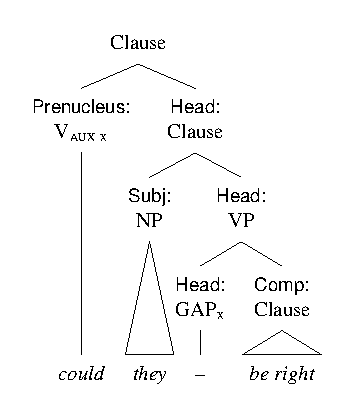
\includegraphics[width=\textwidth]{figures/couldtheyberight.pdf}
    \caption{\textit{Could they be right}: \textsf{Subj}--aux inversion.}
    \label{fig:tree-theycouldberight}
  \end{subfigure}
  \hfill
  \begin{subfigure}[b]{0.48\textwidth}
    \centering
    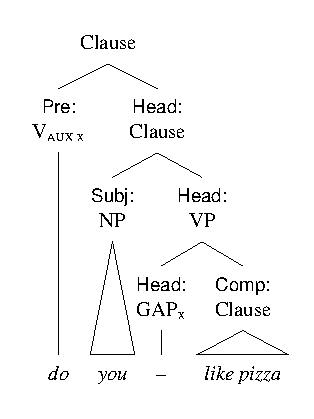
\includegraphics[width=.91\textwidth]{figures/do-you-like-tree.pdf}
    \caption{\textit{Do you like pizza}, with \textit{do} support.}
    \label{fig:do-you-like}
  \end{subfigure}
  \caption{Syntax trees for basic interrogatives.}
  \label{fig:combined-trees}
\end{figure}
%\begin{forest}
%where n children=0{% for each terminal node
%    font=\itshape, 			% italics
%    tier=word          			% align at the "word" tier (bottom)
%  }{%								% no false conditions, so empty
%  },
%[Clause
%	[\Node{Prenucleus}{V\textsubscript{\textsc{aux }x}}[could]]
%	[\Head{Clause}
%		[Section ubj{NP}[they, roof]]
%		[\Head{VP}
%			[\Head{GAP\textsubscript{x}}[--]]
%			[\Comp{Clause}[be right, roof]]
%		]
%	]
%]
%\end{forest}

The first thing to notice about the trees is the \textit{x} subscripts after V\textsubscript{\textsc{aux}} and GAP. Linguists call such a mark a \textsc{co-index}. It's called a \uline{co-}index because it's shared between two (or more) elements, and it's called a co-\uline{index} because, like an index in the back of the book, it points you to something you want to find: if you're wondering where \textit{could} came from, you check the index, and it tells you it came from the position that now says GAP.

The next notable element is the GAP itself, which is a placeholder. The VP, like all phrases, needs a \textsf{Head}, but in this case, the \textsf{Head} is the GAP that's co-indexed to \textit{could}, rather than being a verb, as we would usually expect for the \textsf{Head} of a VP. Such GAPs are more important for linguistic theory than for language teaching, but as we see more gaps in this chapter and others that follow, I expect you'll come to see them as important and useful tools for your own thinking about phrase structure.

Having looked at these two crucial elements, let's go through the tree on the left as a review. Starting at the top, we see that it has an auxiliary verb \textit{could} in \textsf{Prenucleus} function, which is the key element of the basic interrogative clause type. Since \textit{prenucleus} is an ugly, ponderous word used by virtually nobody outside the \textit{CGEL} framework, I will simply call it \textsc{Pre} from now on (there will be a \textsc{Post} later). Be sure to understand that subject--auxiliary inversion does not mean that the subject somehow becomes the auxiliary and vice versa. As the tree shows, the subject remains the subject, and the auxiliary verb appears in the \textsf{Pre} function.

%make sure to introduce Post or remove this

Next, there is the \textsf{Head} clause \textit{they~-- be right}. At first glance, it may seem strange to have a clause as the \textsf{Head} of another clause. But this is an essential aspect of understanding basic interrogatives. In our example, the main clause functions as the \textsf{Head} of the overall interrogative structure. This arrangement is due to the unique positioning of \textit{could} in \textsf{Pre} function. It has to be pre-something, and this shows it as preceding the central clause.

In the tree, the \textsf{Head} clause includes a subject NP (\textit{they}) and a \textsf{Head} VP, represented by the GAP (--) where \textit{could} would normally be. The clause \textit{be right} acts as a \textsf{Complement}, and its internal structure is simplified as a triangle here. I encourage you to sketch this tree yourself to grasp its structure fully. Compare your version with Figure \ref{fig:tree-theycouldberight}, and don't be discouraged if you miss some elements initially. Practice will help you capture all the components accurately.

\subsection{Basic interrogatives with \textit{do} support}

A tree with \textit{do} support looks, structurally, just like one with subject--auxiliary inversion, such as the tree in Figure \ref{fig:tree-theycouldberight}. The tree for the basic interrogative \textit{Do you like pizza?} is shown in Figure \ref{fig:do-you-like}. Again, the auxiliary verb \textit{do} is in \textsf{Pre} function, again the rest of the clause follows as the \textsf{Head}, and again, there's a GAP in the VP.



\subsection{Focused interrogatives with subject focus}\is{interrogative clause|focused|(}

Next is the focused interrogative. Again, we'll start with the easiest case, the one with the interrogative phrase as the subject. The example in Figure \ref{fig:who-plays} is \textit{Who plays the piano?} There's no \textsf{Pre} and no gap, just \textit{who} functioning as the subject. It couldn't be easier, and language learners rarely make mistakes with this clause structure.


\begin{figure}[htbp]
  \centering
  \begin{subfigure}[b]{0.48\textwidth}
    \centering
    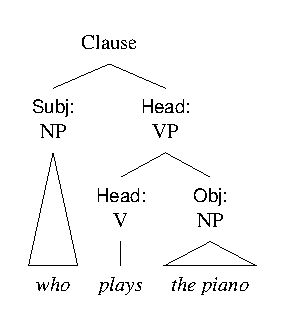
\includegraphics[width=.75\textwidth]{figures/who-plays-tree.pdf}
    \caption{Tree for \textit{who plays the piano}.}
    \label{fig:who-plays}
  \end{subfigure}
  \hfill
  \begin{subfigure}[b]{0.48\textwidth}
    \centering
    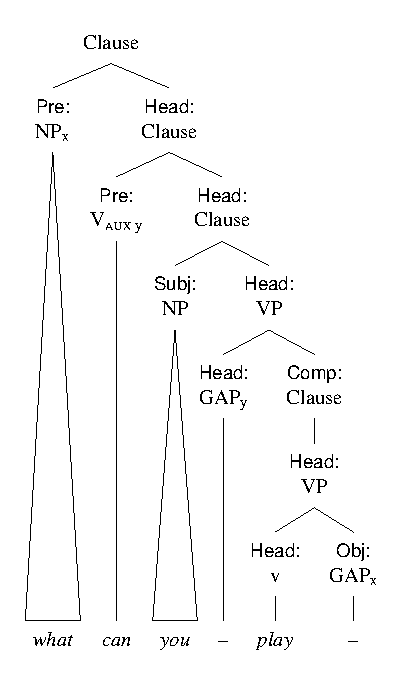
\includegraphics[width=\textwidth]{figures/what-can-you-tree.pdf}
    \caption{Tree for \textit{what can you play}.}
    \label{fig:what-can-you}
  \end{subfigure}
  \caption{Syntax trees for focused interrogatives.}
  \label{fig:combined-trees2}
\end{figure}


%\begin{forest}
%  for tree={
%    l=0.5cm, % Adjusts the level distance
%    s=12cm, % Adjusts the sibling distance
%  },
%where n children=0{% for each terminal node
%    font=\itshape, 			% italics
%    tier=word          			% align at the "word" tier (bottom)
%  }{%								% no false conditions, so empty
%  },
%[Clause
%	[\Node{Pre}{NP\textsubscript{x}}[what, roof]]
%	[\Head{Clause}
%		[\Node{Pre}{V\textsubscript{\textsc{aux }y}}[can]]
%		[\Head{Clause}
%			[Section ubj{NP}[you, roof]]
%			[\Head{VP}
%				[\Head{GAP\textsubscript{y}}[--]]
%				[\Comp{Clause}
%					[\Head{VP}
%						[\Head{v}[play]]
%						[\Obj{GAP\textsubscript{x}}[--]]
%					]
%				]	
%			]
%		]
%	]
%]
%\end{forest}

\subsection{Focused interrogatives with non-subject focus}

When the interrogative phrase (i.e, the focus) is not the subject, then things get more complex and language learners are much more likely to form questions lacking inversion, like \textit{What you can play?} In \textit{What can you play?} in Figure \ref{fig:what-can-you}, there are two constituents in \textsf{Pre} function, two gaps, and two different co-indices \textit{x} and \textit{y}. Each co-index connects the \textsf{Pre} to its relevant gap. 

The functions of the gaps are clearer here. \textit{Play} is a transitive verb, the kind that takes an \textsf{Object}, so there's an \textsf{Object} gap. While we might say informally that \textit{what} is the \textsf{Object} of \textit{play}, that would go against the idea that an \textsf{Object} is a \textsf{Dependent} in the VP, so we give \textit{what} a different function (\textsf{Pre}) but connect it back to the \textsf{Object} through the \textit{x} co-index\is{auxiliary verb!position of|)}\is{auxiliary verb!and inversion|)}\is{auxiliary verb|)}\is{clause!type and inversion|)}\is{do-support@\textit{do}-support|)}\is{fronting!and interrogatives}\is{fronting!of interrogative phrase}\is{fronting!of PP}\is{fronting|)}\is{gap, gapping!and interrogatives|)}\is{interrogative clause!basic vs focused|)}\is{interrogative clause!and inversion|)}\is{interrogative clause|)}\is{inversion!subject--auxiliary|)}\is{subject--auxiliary inversion|)}\is{question!alternative|)}\is{question!yes/no question|)}\is{question|)}\is{response!to question}\is{subject (Subj)!and interrogatives|)}\is{subject (Subj)!and inversion|)}\is{subject (Subj)!|)}\is{answer!right answer|)}\is{answer|)}.
\is{interrogative clause|focused|)}\is{auxiliary do@auxiliary \textit{do}|)}